% SVN info for this file
\svnidlong
{$HeadURL$}
{$LastChangedDate$}
{$LastChangedRevision$}
{$LastChangedBy$}

\chapter{Omotopia}
\labelChapter{omotopia}

\begin{introduction}
	‘‘Molto spesso si è ripetuto che la Geometria è l'arte di ragionare bene su figure mal fatte; in ogni caso queste figure, per non ingannarci, devono soddisfare determinate condizioni; le proporzioni
	possono essere grossolanamente distorte, ma le posizioni relative del
	le varie parti non devono essere interrotte.''
	\begin{flushright}
		\textsc{Henri Poincaré,} dopo aver finito di leggere il già citato libro di Topologia.
	\end{flushright}
\end{introduction}
\lettrine[findent=1pt, nindent=0pt]{F}{inora} abbiamo visto omeomorfismi tra spazi topologici sotto tanti aspetti diversi, definendo così rigorosamente quella che era l'intuizione del magico materiale elastico. Tuttavia, la definizione di omeomorfismo è molto rigida e possiamo osservare delle ‘‘\textit{equivalenze di forma}'' che non riesce pertanto a descrivere.\\
Ad esempio, si possono considerare \textit{equivalenti} figure con lo stesso numero di buchi. Sotto questo punto di vista, le figure corrispondenti alla lettera \textsf{\textbf{O}} e  \textsf{\textbf{P}} sono \textit{equivalenti}, dato che hanno entrambe un solo buco, mentre \textsf{\textbf{X}} non lo è perché non ne ha. Allo stesso tempo, nessuna di queste è \textit{omeomorfa} all'altra: infatti, se togliamo dalle tre figure un punto come il nodo di raccordo delle ‘‘stanghette'' (o per \textsf{\textbf{O}} un punto qualunque), otteniamo per \textsf{\textbf{O}} una componente connessa, per \textsf{\textbf{P}} due e per \textsf{\textbf{X}} ben quattro distinte.\\
Preceduto da un approfondimento sulle componenti connesse e c.p.a., nel presente capitolo formalizzeremo questo tipo di equivalenza più debole e allo stesso tempo più ampia: l'\textbf{omotopia}.
\section{Lemma di incollamento}
\begin{lemma}{}[Lemma di incollamento]\label{lemmaincollamento}
Siano $X,\ Y$ spazi topologici e $X=A\cup B$. Siano $\funct{}[f]{A}{Y}$ e $\funct{}[g]{B}{Y}$ continue tali che $f\left(x\right)=g\left(x\right)\ \forall x\in A\cap B$, cioè $f_{\mid A\cap B}=g_{\mid A\cap B}$. Consideriamo l'\textbf{incollamento}\index{incollamento} $\funct{}[h]{X}{Y}$ definito da
	\begin{equation*}
		h\left(x\right)=
		\begin{cases}
			f\left(x\right)& x\in A\\
			g\left(x\right)& x\in B
		\end{cases}
	\end{equation*}
	Se $A$ e $B$ sono entrambi aperti o entrambi chiusi in $X$, allora $h$ è continua.
\end{lemma}
\begin{proof}{n}
	Supponiamo $A$ e $B$ aperti. Sia $U\subseteq Y$ aperto. Allora
	\begin{equation*}
		h^{-1}\left(U\right)=\underbrace{f^{-1}\left(U\right)}_{\subseteq A}\cup \underbrace{g^{-1}\left(U\right)}_{\subseteq B}.
	\end{equation*}
Essendo $f,\ g$ continue, segue che $f^{-1}\left(U\right)$ è aperto in $A$ e $g^{-1}\left(U\right)$ è aperto in $B$. In quanto $A,\ B$ aperti, per definizione di aperto del sottospazio\footnote{Poiché un aperto del sottospazio è dato dall'intersezione del sottospazio con un aperto di $X$, se abbiamo che anche il sottospazio è aperto di $X$, l'intersezione è aperta: in questo caso ogni aperto del sottospazio è anche aperto di $X$.} $f^{-1}\left(U\right)$ e $g^{-1}\left(U\right)$ sono aperti su $X$ e pertanto $h^{-1}\left(U\right)$ aperto. Il caso di $A$ e $B$ chiusi è analogo.\qedhere
\end{proof}
\section{Componenti connesse e componenti c.p.a.}
Riprendiamo la trattazione delle componenti connesse e c.p.a. introdotte nel \autoref{chap:Connessocompatto}.
\begin{definition}{}[Componente connessa]
	Una \textbf{componente connessa}\index{componente!connessa} di $X$ spazio topologico è un sottospazio $C\subseteq X$ \textit{connesso massimale}, ossia per ogni $A$ connesso tale per cui $C\subseteq A\subseteq X$ si ha $C=A$.
\end{definition}
\begin{remark}{pn}~{}
\begin{itemize}
	\item Le componenti connesse formano una \textit{partizione} di $X$.
	\item Se $x\in X$ si può definire la componente connessa che contiene $x$:
	\begin{equation*}
		C\left(x\right)\coloneqq\bigcup\Set{C\subseteq X | x\in C,\ C\ \text{connesso}}.
	\end{equation*}
\item Le componenti connesse possono essere viste come \textit{classi di equivalenza} per la seguente relazione su $ X $: presi $x,y\in X$,
	\begin{equation*}
		x\sim_C y\iff \exists C\subseteq X\ \text{connesso}\ \colon x,\ y\in C.
	\end{equation*}
\end{itemize}
\end{remark}
\begin{proof}{n}
Mostriamo che la relazione è di equivalenza:
\begin{itemize}
\item \textit{Riflessività}: poiché $\left\{x\right\}$ è sempre un connesso, vale $x\sim_C x$.
\item \textit{Simmetria}: ovvia dalla definizione.
\item \textit{Transitività}: supponiamo $x\sim_C y,\ y\sim_C z$. Allora esistono $C,\ D\subseteq X$ connessi tali che $x,\ y\in C$ e $y,\ z\in D$. Allora $C\cup D$ contiene sia $x$ che $z$; inoltre, essendo $y\in C\cap D$ si ha $C\cap D\neq \emptyset$, dunque $C\cup D$ è un connesso: vale $x\sim_C z$.
\end{itemize}
Dimostriamo che la classe di equivalenza $C_0=\left[x\right]$ di $\sim$ coincide con la componente connessa $C$ contente $x$, ossia $C=C(x)=C_0$.\\
$\rightinclude$Per ogni $x, y\in C$ per definizione di $\sim$ si ha $x\sim_C y$, ossia $C\subseteq C_0=[x]=[y]$.\\
$\leftinclude$Sia $z\in C_0=\left[x\right]$, dove $x\in C$ componente connessa. Allora $x\sim_C z$, dunque deve esistere $T\subseteq X$ connesso tale che $x,\ z\in T$. Consideriamo $C\cup T$: poiché sono entrambi connessi e $x\in C\cap T \neq \emptyset$, segue che $C\cup T$ è ancora connesso. In quanto $C$ è componente connessa, poiché $C\subseteq C\cup T$, per massimalità abbiamo $C=C\cup T$, cioè $T\subseteq C$. Allora $z\in C$; per arbitrarietà di $z$ ricaviamo che $C_0\subseteq C$.\qedhere
\end{proof}
\begin{definition}{}[Componente c.p.a.]
Una \textbf{componente c.p.a.}\index{componente!c.p.a.} di $X$ è una classe di equivalenza per la seguente relazione su $ X $: presi $x,y\in X$,
	\begin{equation*}
	x\sim_A y\iff \exists \funct{}[\alpha]{I}{X}\ \text{cammino continuo}\colon \alpha\left(0\right)=x,\ \alpha\left(1\right)=y.
\end{equation*}
\end{definition}
\begin{proof}{n}
	Mostriamo che sia una relazione di equivalenza:
	\begin{itemize}
		\item \textit{Riflessività}: poiché esiste sempre il \textbf{cammino costante}\index{cammino!costante}
		\begin{equation}
			\funct{}[c_x]{I}{X}[t][x]
		\end{equation}
		nel punto $x$, $x\sim_A x$ è vero.
		\item \textit{Simmetria}: se $x\sim_A y$ sappiamo che esiste un cammino $\funct{}[\alpha]{I}{X}$ tale per cui $\alpha\left(0\right)=x,\ \alpha\left(1\right)=y$. Possiamo definire il \textbf{cammino inverso}\index{cammino!inverso}
		\begin{equation}
			\funct{}[\overline{\alpha}]{I}{X}[t][\alpha\left(1-t\right)].
		\end{equation}
	\begin{itemize}
		\item $\overline{\alpha}$ è continuo, perché composizione di applicazioni continue:\\
		\begin{center}
			\begin{tikzcd}
				I \arrow[r]          & I \arrow[r, "\alpha"]  & X                      \\[-25pt]
				t \arrow[r, maps to] & 1-t \arrow[r, maps to] & \alpha\left(1-t\right)
			\end{tikzcd}
		\end{center}
	\item $\overline{\alpha}\left(0\right)=\alpha\left(1\right)=y,\ \overline{\alpha}\left(1\right)=\alpha\left(0\right)=x$.
	\end{itemize}
Allora il cammino $\overline{\alpha}$ definisce $y\sim_A x$.
		\item \textit{Transitività}: supponiamo $x\sim_A y,\ y\sim_A z$. Allora esistono cammini $\funct{}[\alpha,\ \beta]{I}{X}$ tali che $\alpha\left(0\right)=x,\ \alpha\left(1\right)=y, \beta\left(0\right)=y,\ \beta\left(1\right)=z$. Usando la \textbf{giunzione di cammini}\index{cammino!giunzione di cammini}
	\begin{equation*}
	\left(\alpha\ast\beta\right)\left(t\right)=\begin{cases}
		\begin{array}{lc}
					\alpha\left(2t\right) & \text{se }0\leq t\leq \frac{1}{2}\\
			\beta\left(2t-1\right) & \text{se }\frac{1}{2}\leq t\leq 1	
		\end{array}
	\end{cases}
\end{equation*}
otteniamo che
\begin{align*}
	\left(\alpha\ast\beta\right)\left(0\right)&=\alpha\left(0\right)=x\\
	\left(\alpha\ast\beta\right)\left(1\right)&=\beta\left(1\right)=z.
\end{align*}
Poiché $\alpha\ast\beta$ soddisfa le ipotesi del lemma di incollamento, esso è continua e collega con un cammino unico $x$ e $z$, dunque vale $x\sim_A z$.\qedhere
	\end{itemize}
\end{proof}
\begin{remark}{pn}~{}
	\begin{enumerate}
		\item Le componenti c.p.a. formano una partizione di $X$.
		\item Sia $C\subseteq X$ un sottospazio c.p.a. per cui vale che se esiste $A$ c.p.a. tale che $C\subseteq A\subseteq X$ allora $C=A$. Ne consegue che $C$ è una componente c.p.a. -- in altre parole, le componenti c.p.a. sono sottospazi c.p.a. massimali.
		\item In generale le componenti c.p.a. non sono né aperte né chiuse.
		\item Se $A$ è una componente c.p.a., allora $A$ è c.p.a. e dunque \textit{connessa}: $A$ è interamente contenuta in una componente connessa, cioè le componenti connesse sono unioni di componenti c.p.a..
	\end{enumerate}
\end{remark}
\begin{proof}{n}
	Dimostriamo il punto $2$. Supponiamo per assurdo che esista $z\in X\setminus C$ tale che esista un cammino $\alpha$ tra un punto $x\in C$ e $z$. Definiamo $A\coloneqq C\cup \img\alpha$, con $\img\alpha$ il percorso di $\alpha$ in $X$. Si ha che $A$ è c.p.a., essendo esso unione di spazi c.p.a.: $C$ lo è per ipotesi e $\img\alpha$ lo è banalmente per definizione. In particolare, $A\subseteq C$, dunque per ipotesi $A=C$. Ma allora $z\in A=C$, il che è assurdo! Segue che \textit{non} esiste alcun cammino con punti esterni a $C$, dunque $C$ è componente c.p.a. di $X$.\qedhere
\end{proof}
\begin{example}{n}
	Ricordiamo l'esempio della \textit{pulce e il pettine}, cioè lo spazio
	\begin{gather*}
		X=Y\cup \{p\}\subseteq\R^2\ \text{con}\ Y=\left(I\times \left\{0\right\}\right)\cup \bigcup_{r\in\Z}\left(\left\{r\right\}\times I\right)\ \text{e}\ p=\left(\frac{\sqrt{2}}{2},\ 1\right).
	\end{gather*}
Questo spazio è connesso ma non c.p.a.. Infatti, le componenti c.p.a. sono due: $Y$ e $\left\{p\right\}$.
\end{example}
\section{Omotopia tra funzioni continue}
\begin{intuitively}{n}
	Dati due spazi topologici $X,\ Y$ e due funzioni $\funct{}[f,g]{X}{Y}$, si ha un'\textbf{omotopia} tra le due funzioni se una funzione può essere ‘‘\textit{deformata in modo continuo}'' nell'altra (e viceversa). Per far ciò vogliamo trovare una famiglia di funzioni $\left\{f_t\right\}_{t\in\left[0,\ 1\right]}$ tale che ogni funzione $\funct{}[f_t]{X}{Y}$ sia continua e vari ‘‘\textit{con continuità}'' al variare di $t\in\left[0,\ 1\right]$ fra $f_0=f$ e $f_1=g$.
\end{intuitively}
\begin{definition}{}[Omotopia]
	Due funzioni continue $\funct{}[f,\ g]{X}{Y}$ si dicono \textbf{omotope} se esiste una funzione $\funct{}[F]{X\times I}{Y}$ \textit{continua} tale che $F\left(x,0\right)=f\left(x\right)$ e $F\left(x,1\right)=g\left(x\right)$ per ogni $x\in X$. La funzione $F$ è detta \textbf{omotopia}\index{omotopia} tra $f$ e $g$.
\end{definition}
\begin{notation}{n}
	Denotiamo le funzioni omotope con $f\sim g$. Inoltre, denotiamo gli elementi della famiglia di funzioni $\left\{f_t\right\}_{t\in\left[0,\ 1\right]}$ nel seguente modo:
	\begin{equation*}
		\forall t,\ f_t\coloneqq \funct{}[F(\cdot, t)]{X}{Y}\ \colon f_0=f,\ f_1=g
	\end{equation*}
\end{notation}
\begin{remark}{n}
Dato un \textit{segmento} $\overline{AB}$, la funzione
\begin{equation*}
	\funct{}{I}{\overline{AB}}[t][tA+\left(1-t\right)B]
\end{equation*}
è biunivoca e, in particolare, è omeomorfismo.
\end{remark}
\begin{example}{n}\label{convessoomotope}
	Dato un sottospazio $Y\subseteq \R^n$ \textit{convesso}, per ogni spazio topologico $X$ e per ogni coppia di funzioni $\funct{}[f, g]{X}{Y}$ continue, allora $f$ e $g$ sono \textit{omotope}.
\end{example}
\begin{proof}{n}
	L'omotopia è
	\begin{equation*}
		\funct{}[F]{X\times I}{Y}[\left(x,\ t\right)][\left(1-t\right)f\left(x\right)+tg\left(x\right)].
	\end{equation*}
\begin{itemize}
	\item $F$ è ben definita. Se $x\in X$, abbiamo $f\left(x\right),\ g\left(x\right)\in Y$ convesso: esiste allora il segmento $\overline{f\left(x\right)g\left(x\right)}\subseteq Y$, cioè $\left(1-t\right)f\left(x\right)+tg\left(x\right)\in Y, \forall x\in X,\ t\in I$.
	\item $F$ è continua perché composizione di funzioni continue:
	\begin{center}
		\begin{tikzcd}
			X\times I \arrow[r]            & Y\times Y\times I\subseteq \R^{2n+1} \arrow[r]           & Y\subseteq \R^n                            \\[-25pt]
			{\left(x,\ t\right)} \arrow[r, maps to] & {\left(f\left(x\right),\ g\left(x\right),\ t\right)} \arrow[r, maps to] & \left(1-t\right)f\left(x\right)+tg\left(x\right)
		\end{tikzcd}
	\end{center}
\item $F\left(x,\ 0\right)=f\left(x\right),\ F\left(x,\ 1\right)=g\left(x\right),\ \forall x\in X$.\qedhere
\end{itemize}
\end{proof}
\begin{remark}{n}\label{omotopiasegmento}
	Sia $Y\subseteq \R^n$ non necessariamente convesso e $\funct{}[f, g]{X}{Y}$ continue tali che $\overline{f\left(x\right)g\left(x\right)}\subseteq Y,\ \forall x\in X$. Allora $f$ è omotopa a $g$ con la stessa omotopia $F$ definita qui sopra nel caso di $Y$ convesso.
\end{remark}
\begin{warning}{n}
Nel parlare di omotopie è estremamente importante verificare che siano ben definite! Infatti, prendiamo ad esempio $Y=S^1\subseteq \R^2$ e le funzioni costanti in $p$ e in $q$, rispettivamente
\begin{equation*}
	\funct{}[f]{X}{S^1}[x][p]\qquad\funct{}[g]{X}{S^1}[x][q].
\end{equation*}
Considerata
\begin{equation*}
	\funct{}[F]{X\times I}{\R^2}[\left(x,y\right)][\left(1-t\right)f\left(x\right)+tg\left(x\right)=\left(1-t\right)p+tq],
\end{equation*}
essa \textit{non} è ben definita in $Y$: presi due punti della sfera $S^1$ il segmento non è \textit{mai} contenuto in essa!
\end{warning}
\begin{lemma}{}[Omotopia è relazione di equivalenza]
	Siano $X,\ Y$ due spazi topologici. L'omotopia è una \textit{relazione di equivalenza} sull'insieme delle funzioni continue da $X$ e $Y$.
\end{lemma}
\begin{proof}{n}~{}
	\begin{itemize}
		\item \textit{Riflessività}: sia $\funct{}[f]{X}{Y}$ continua. Consideriamo
		\begin{equation*}
			\funct{}[F]{X\times I}{Y}[\left(x,\ t\right)][f\left(x\right)].
		\end{equation*}
		\begin{itemize}
			\item È continua perché lo è $f$;
			\item $F\left(x,0\right)=F\left(x,1\right)=f\left(x\right)\ \forall x\in X$.
		\end{itemize}
		Allora $f\sim f$.
		\item \textit{Transitività}: supponiamo $f\sim g$, cioè esiste $\funct{}[F]{X\times I}{Y}$ tale che $F\left(x,0\right)=f\left(x\right)$ e $F\left(x,1\right)=g\left(x\right)$, per ogni $x\in X$. Consideriamo
	\begin{equation*}
		\funct{}[G]{X\times I}{Y}[\left(x,\ t\right)][F\left(x,1-t\right)].
	\end{equation*}
	\begin{itemize}
		\item È continua perché composizione di funzioni continue.
		\item $G\left(x,0\right)=F\left(x,1\right)=g\left(x\right)$ e $G\left(x,1\right)=F\left(x,0\right)=f\left(x\right),$ per ogni $x\in X$.
	\end{itemize}
Allora $g\sim f$.
\item \textsc{Transitiva}: siano $\funct{}[f, g, h]{X}{Y}$ continue, $f\sim g$ e $g\sim h$, cioè esistono $\funct{}[F]{X\times I}{Y}$ e $\funct{}[G]{X\times I}{Y}$ con
\begin{equation*}
		F\left(x,0\right)=f\left(x\right)\qquad	F\left(x,1\right)=g\left(x\right)\\
		G\left(x,0\right)=g\left(x\right)\qquad	G\left(x,1\right)=h\left(x\right)
\end{equation*}
per ogni $x\in X$. Consideriamo $\funct{}[H]{X\times I}{Y}$ definita come
\begin{equation*}
	H\left(x,t\right)=\begin{cases}
		\begin{array}{lc}
			F\left(x,2t\right) & t\in\left[0,\ \frac{1}{2}\right] \\
			G\left(x,2t-1\right) & t\in\left[\frac{1}{2},\ 1\right]
		\end{array}	
	\end{cases}
\end{equation*}
\begin{itemize}
	\item $H$ è continua per il lemma di incollamento:
	\begin{itemize}
		\item È ben definita per $t=\frac{1}{2}$.
		\item $H$ è continua separatamente su $X\times \left[0,\ \frac{1}{2}\right]$ e $X\times \left[\frac{1}{2},\ 1\right]$, entrambi chiusi.
	\end{itemize}
\item $H\left(x,0\right)=F\left(x,0\right)=f\left(x\right),\ H\left(x,1\right)=G\left(x,1\right)=h\left(x\right)$ per ogni $x\in X$.
\end{itemize}
Allora $f\sim h$.\qedhere
\end{itemize}
\end{proof}
\begin{lemma}{}[Composizione di omotopie; Manetti, 10.13]\label{compomotop}
Siano $X,\ Y,\ Z$ spazi topologici e siano $\funct{}[f_1, f_2]{X}{Y}$ continue ed omotope, $\funct{}[g_1, g_2]{Y}{Z}$ continue ed omotope. Allora $\funct{}[g_1\circ f_1, g_2\circ f_2]{X}{Z}$ sono omotope, ossia
\begin{equation*}
	f_1\sim f_2,\ g_1\sim g_2\implies g_1\circ f_1\sim g_2\circ f_2
\end{equation*}
\end{lemma}
\begin{proof}{n}
	Sappiamo che:
	\begin{itemize}
		\item esiste $\funct{}[F]{X\times I}{Y}$ continua con $F\left(x,0\right)=f_1\left(x\right),\ F\left(x,1\right)=f_2\left(x\right), \forall x\in X$.
		\item esiste $\funct{}[G]{Y\times I}{Z}$ continua con $G\left(y,0\right)=g_1\left(y\right),\ G\left(y,1\right)=g_2\left(y\right), \forall y\in Y$.
	\end{itemize}
Sia
\begin{equation*}
	\funct{}[H]{X\times I}{Z}[\left(x,\ t\right)][G\left(F\left(x,t\right),t\right)]
\end{equation*}
\begin{itemize}
	\item $H$ è continua perché composizione di funzioni continue.
	\item $H\left(x,0\right)=G\left(F\left(x,0\right),0\right)=G\left(f_1\left(x\right),0\right)=g_1\left(f_1\left(x\right)\right),\ \forall x\in X$.
	\item $H\left(x,1\right)=G\left(F\left(x,1\right),1\right)=G\left(f_2\left(x\right),1\right)=g_2\left(f_2\left(x\right)\right),\ \forall x\in X$.
\end{itemize}
Allora $H$ è l'omotopia cercata.\qedhere
\end{proof}
\section{Equivalenza omotopica}
Dati due spazi topologici, diciamo che essi sono \textit{omeomorfi} se esistono due omeomorfismi l'uno l'inverso dell'altro. Proviamo ora ad analizzare il caso in cui indeboliamo la relazione tramite l'\textbf{omotopia}.
\begin{definition}{}[Omotopicamente equivalenti]
	Siano $X,\ Y$ due spazi topologici. $X$ e $Y$ sono \textbf{omotopicamente equivalenti}\seeonlyindex{omotopicamente equivalenti}{tipo di omotopia}, o che hanno lo stesso \textbf{tipo di omotopia}\index{tipo di omotopia}, se esistono due applicazioni continue $\funct{}[f]{X}{Y}$ e $\funct{}[g]{Y}{X}$ tali che $g\circ f\sim Id_X$ e $f\circ g\sim Id_Y$. In tal caso, $f$ e $g$ si dicono \textbf{equivalenze omotopiche}\index{equivalenze omotopiche}.
\end{definition}
\begin{remark}{pn}~{}
\begin{enumerate}
	\item Se $X$ e $Y$ sono \textit{omeomorfi}, allora sono anche \textit{omotopicamente equivalenti}.
	\item Consideriamo $X=\R^n$ in topologia Euclidea e $Y=\left\{\ast\right\}$, con $\ast$ un punto. Allora $X$ e $Y$ sono omotopicamente equivalenti.
\end{enumerate}
\end{remark}
\begin{proof}{n}~{}
	\begin{enumerate}[label=\Roman*]
		\item L'omotopia è una relazione riflessiva, dunque se abbiamo $h=k$ e $h\sim h$, allora $h\sim k$. Nel caso di un omeomorfismo, preso $f$ con inverga $g$, si ha
		\begin{equation*}
			g\circ f=Id_X\quad f\circ g=Id_Y\implies g\circ f\sim Id_X\quad f\circ g\sim Id_Y.
		\end{equation*}
	\item Consideriamo
	\begin{equation*}
		\funct{}[f]{\R^n}{Y=\left\{\ast\right\}}[\mathbb{x}][\ast]\qquad\funct{}[g]{Y=\left\{\ast\right\}}{\R^n}[\ast][g\left(\ast\right)=\mathbf{0}]
	\end{equation*}
$f$ e $g$ sono \textit{continue}, inoltre:
	\begin{align*}
		\funct{}[f\circ g]{Y=\left\{\ast\right\}}{Y=\left\{\ast\right\}}[\ast][\ast]&\implies f\circ g= Id_Y\\
		\funct{}[g\circ f]{\R^n}{\R^n}[\mathbf{x}][\mathbf{0}]&\implies g\circ f=O_{\R^n}\ \text{(applicazione nulla)}
	\end{align*}
Poiché $f\circ g= Id_Y$, per 1. allora $f\circ g\sim Id_Y$. Abbiamo che $g\circ f=O_{\R^n}$ è omotopa a $Id_{\R^n}$, in quanto $\R^n$ è \textit{convesso} e due applicazioni continue a valori in $\R^n$ sono sempre omotope, come dimostrato nell'esempio a pag. \pageref{convessoomotope}. Una di queste, ad esempio, è la seguente:
\begin{equation*}
\funct{}[F]{\R^n\times I}{\R^n}[\left(x,t\right)][t\cdot \mathbf{x}]..
\end{equation*}
\begin{itemize}
	\item $F$ è continua.
	\item $F\left(\mathbf{x},0\right)=\overline{0}=\left(g\circ f\right)\left(x\right)$.
	\item $F\left(\mathbf{x},1\right)=\mathbf{x}=Id_{\R^n}\left(\mathbf{x}\right)$.\qedhere
\end{itemize}
\end{enumerate}
\end{proof}
\begin{warning}{n}
	Se $n>0$, $\R^n$ e $\left\{\ast\right\}$ \textit{non} sono omeomorfi, dato che \textit{non} possono essere in corrispondenza biunivoca.
\end{warning}
\begin{remark}{n}
	\textit{Essere omotopicamente equivalenti} è una relazione di equivalenza sull'insieme degli spazi topologici.
\end{remark}
\begin{proof}{n}~{}
	\begin{itemize}
	\item \textit{Riflessività}: $X\sim X$ se e solo se esistono $f,\ g$ continue per cui $g\circ f\sim Id_X,\ f\circ g\sim Id_X$. Ponendo $f\coloneqq Id_X\eqqcolon g$ vale banalmente $g\circ f=f\circ g=Id_X\sim Id_X$.
	\textit{Simmetria}: ovvia dalla definizione.
	%\item \textit{Simmetria}: da $X\sim Y$ sappiamo che esistono $\funct{}[f]{X}{Y},\ \funct{}[g]{Y}{X}$ continue per cui $g\circ f\sim Id_X,\ f\circ g\sim Id_Y$; se vogliamo mostrare $Y\sim X$ dobbiamo cercare $\funct{}[h]{Y}{X},\ \funct{}[k]{X}{Y}$ per cui $k\circ h\sim Id_Y,\ h\circ k\sim Id_X$. Ponendo $h\coloneqq g$ e $k\coloneqq f$, esse soddisfano la richiesta.
	\item \textit{Transitività}: da $X\sim Y$ e $Y\sim Z$ si hanno
	\begin{itemize}
		\item $\funct{}[f]{X}{Y},\ \funct{}[g]{Y}{X}$ continue tali che $g\circ f\sim Id_X,\ f\circ g\sim Id_Y$.
			\item $\funct{}[h]{Y}{Z},\ \funct{}[k]{Z}{Y}$ continue tali che $k\circ h\sim Id_Y,\ h\circ k\sim Id_Z$.
	\end{itemize}
	Vogliamo trovare $\funct{}[a]{X}{Z},\ \funct{}[b]{Z}{X}$ continue tali che $b\circ a\sim Id_X,\ a\circ b\sim Id_Z$. Se definiamo
	\begin{equation*}
		a\coloneqq \funct{}[h\circ f]{X}{Z}\qquad b\coloneqq \funct{}[g\circ k]{Z}{X}.
	\end{equation*}
	Si ha allora
	\begin{align*}
		b\circ a&=\left(g\circ k\right)\circ\left(h\circ f\right)=g\circ \left(k\circ h\right)\circ f\\
		a\circ b&=\left(h\circ f\right)\circ \left(g\circ k\right)=h\circ\left(f\circ g\right)\circ k.
	\end{align*}
	Dalla composizione di funzioni omotope
	\begin{equation*}
		\begin{array}{cccccc}
			f\sim f & & & &\\
			& \implies & \left(k\circ h\right)\circ f\sim Id_y\circ f& &\\
			k\circ h\sim Id_Y& & &\implies &g\circ \left(k\circ h\right)\circ f\sim g\circ Id_y\circ f. \\
			& & g\sim g & &\\
		\end{array}
	\end{equation*}
	Osserviamo che
	\begin{equation*}
		b\circ a = g\circ \left(k\circ h\right)\circ f \sim g\circ Id_Y\circ f = g\circ f \sim Id_X
	\end{equation*}
e quindi $b\circ a\sim Id_X$. In modo analogo
\begin{equation*}
	\begin{array}{cccccc}
		k\sim k & & & &\\
		& \implies & \left(f\circ g\right)\circ k\sim Id_y\circ k& &\\
		f\circ g\sim Id_Y& & &\implies &h\circ \left(f\circ g\right)\circ k\sim g\circ Id_y\circ f \\
		& & h\sim h & &\\
	\end{array}
\end{equation*}
fa si che
\begin{equation*}
	a\circ b = h\circ \left(f\circ g\right)\circ k \sim h\circ Id_Y\circ k =h\circ k \sim Id_Z
\end{equation*}
da cui si ha $a\circ b\sim Id_Z$.\qedhere
\end{itemize}
\end{proof}
\subsection{Spazi contraibili}
\begin{definition}{}[Spazio contraibile]
	Uno spazio topologico è \textbf{contraibile}\index{spazio!contraibile} o \textit{contrattile}\seeonlyindex{spazio!contrattile}{spazio!contraibile} se ha lo stesso tipo di omotopia di un punto.
\end{definition}
\begin{example}{pn}~{}
	\begin{enumerate}
		\item $\R^n$ è contraibile: si veda l'osservazione precedente.
		\item Dall'esempio precedente, per transitività del tipo di equivalenza, si può affermare che \textit{tutti} i $\R^n$ sono tutti omotopicamente equivalenti tra di loro.
		\item Ogni sottospazio $X\subseteq \R^n$ \textit{convesso} è contraibile.
		\item Ogni sottospazio $X\subseteq \R^n$ \textit{stellato} è contraibile.
	\end{enumerate}
\end{example}
\begin{proof}{n}
	Dimostriamo l'esempio $4)$: l'esempio $3)$ è automaticamente dimostrato perché un convesso è stellato per ogni suo punto.	Sia $P_0\in X$ il punto rispetto al quale $X$ è stellato e consideriamo l'inclusione del singoletto $\left\{P_0\right\}$ in $X$ e la funzione costante da $X$ al punto, entrambe costanti:
	\begin{equation*}
		\funct{i}[i]{\left\{P_0\right\}}{X}\qquad \funct{}[g]{X}{\left\{P_0\right\}}
	\end{equation*}
\begin{itemize}
	\item  La funzione
	\begin{equation*}
		\funct{}[g\circ i]{\left\{P_0\right\}}{\left\{P_0\right\}}
	\end{equation*}
	è pari all'identità $Id_{\left\{P_0\right\}}$ del singoletto e dunque ovviamente omotopa ad essa.
	\item La funzione
	\begin{equation*}
		\funct{}[\phi\coloneqq i\circ g]{X}{X}[P][P_0]
	\end{equation*}
	è costante; vogliamo dimostrare che $\phi$ è omotopa a $Id_X$. Siccome $X$ è stellato rispetto a $P_0$, per ogni $P\in X$ si ha $\overline{PP_0}\subseteq X$. Allora definiamo la funzione
	\begin{equation*}
		\funct{}[F]{X\times I}{X}[\left(P,\ t\right)][tP+\left(1-t\right)P_0].
	\end{equation*}
Ha senso definire ciò proprio perché su $X\subseteq \R^n$ ci sono le operazioni di somma e prodotto per scalari. Oltre ad essere ben definita per quanto detto prima, $F$ è continua e $F\left(P,0\right)=P_0=\phi\left(0\right)$, $F\left(P,1\right)=P=Id_X\left(P\right)$. Si ha l'omotopia cercata.\qedhere
\end{itemize}
\end{proof}
\begin{example}{n}
$\R^2\setminus\left\{\left(0,\ 0\right)\right\}$ non è né convesso, né stellato.
\end{example}
\begin{lemma}{n}[$X$ contraibile implica $X$ c.p.a.]
\end{lemma}
\begin{proof}{n}
	Con il seguente diagramma ricordiamo le funzioni in gioco con la contraibilità:
\begin{center}
	\begin{tikzcd}
		\left\{\ast\right\} \arrow[r, "g", bend left] & X \arrow[l, "f\text{ (costante)}", bend left]
	\end{tikzcd}
\end{center}
Necessariamente dobbiamo mappare $g$ ad un punto di $x_0\in X$. Il singoletto e $X$ sono in equivalenze omotopica, in particolare da ciò si ha una funzione costante in $x_0$:
\begin{equation*}
	\funct{}[\phi\coloneqq g\circ f]{X}{X}[x][x_0]
\end{equation*}
Poiché $f$ e $g$ sono in equivalenza omotopica, si ha che $\phi\sim Id_X$, cioè esiste un omotopia fra le due funzioni:
\begin{equation*}
	\funct{}[F]{X\times I}{X}\text{ continua}\ \colon F\left(x,0\right)=\phi\left(x\right)=x_0,\ F\left(x,1\right)=Id_X\left(x\right)=x,\ \forall x\in X
\end{equation*}
Fissato $x\in X$, sia $\funct{}[\alpha]{I}{X}$ dato da $\alpha\left(t\right)\coloneqq F\left(x,t\right)$:
\begin{itemize}
	\item $\alpha$ è continua perché lo è $F$.
	\item $\alpha\left(0\right)=F\left(x,0\right)=x_0$, $\alpha\left(1\right)=F\left(x,1\right)=x$.
\end{itemize}
Segue che $\alpha$ è un cammino da $x_0$ a un qualunque punto $x$ in $X$, dunque $X$ è c.p.a..\qedhere
\end{proof}
\begin{exercise}{n}
Se $X$ e $Y$ sono omotopicamente equivalenti, allora:
\begin{enumerate}
\item $X$ è c.p.a. $\iff Y$ è c.p.a..
\item $X$ è connesso $\iff Y$ è connesso.
\end{enumerate}
\end{exercise}
\begin{proof}{n} Siano $f,\ g$ le equivalenze omotopiche.
	\begin{center}
		\begin{tikzcd}
			X \arrow[r, "f", bend left] & Y \arrow[l, "g", bend left]
		\end{tikzcd}
	\end{center}
	\begin{enumerate}[label=\Roman*]
		\item 
$\rightimplies$Considerato $f\circ g\sim Id_Y$, l'omotopia tra le due funzioni è tale per cui:
\begin{equation*}
	\funct{}[F]{Y\times I}{Y}\ \colon F(y,0)=f(g(y)), F(y,1)=y,\ \forall y\in Y
\end{equation*}
Possiamo usare $F$ per costruire, ad $y\in Y$ fissato, un arco in $Y$ che collega $y$ ad un punto di $f\left(X\right)\subseteq Y$. Infatti, consideriamo $\funct{}[\alpha]{I}{Y}$ dato da $\alpha\left(t\right)=F\left(y,t\right)$:
\begin{itemize}
	\item $\alpha$ è continua perché lo è $F$.
	\item $\alpha(0)=F(y,0)=f(g(y))\in f(X),\ \alpha(1)=F(y,1)=y$.
\end{itemize}
Supponendo $X$ c.p.a., allora $f\left(X\right)$ è c.p.a. Per i ragionamenti appena fatti abbiamo che ogni punto di $Y$ ha un arco che lo collega ad un punto di $f\left(X\right)$; presi due punti di $Y$ possiamo ricondurci sempre a due punti (\textit{non} necessariamente distinti) in $f\left(X\right)$ che possiamo collegare con un cammino $\gamma$ opportuno in quanto $f\left(X\right)$ c.p.a.. Per giunzione di cammini possiamo collegare con un cammino in $Y$ i due punti di $Y$, pertanto per arbitrarietà dei punti scelti $Y$ è c.p.a..\\
$\leftimplies$Supponendo che $Y$ sia c.p.a., applicando all'equivalenza omotopica $g\circ f\sim Id_X$ un procedimento analogo a $\rightimplies$si ha che $X$ è c.p.a.
%\footnote{In realtà è sufficiente, per i ragionamenti visti sopra, dire che se $X$ e $Y$ sono omotopicamente equivalenti, allora $X$ è c.p.a. $\iff$ $f\left(X\right)$ è c.p.a..}. (siamo sicuri?)
\item $\rightimplies$Sia $X$ connesso. Sia $Y=\bigcup_i Y_i$ la scomposizione di $Y$ in componenti connesse. Poiché $X$ è connesso, allora $f\left(X\right)\subseteq Y_i$ per un certo $i$. Allora $\left(f\circ g\right)\left(Y\right)\subseteq Y_i$. Consideriamo l'omotopia $\funct{}[F]{Y\times I}{Y}$ associata a $f\circ g\sim Id_Y$. Come nel punto I possiamo definire per ogni punto di $Y$ un cammino $\alpha\left(t\right)=F\left(y,t\right)$ tra $y$ e un punto di $f\left(X\right)$. Poichè per ogni $y\in Y$ abbiamo $\alpha\left(0\right)\subseteq Y_i$ per un certo $i$ e $I$ è c.p.a., allora $\alpha\left(I\right)\subseteq Y_i$. Pertanto, anche $F\left(X\times I\right)\subseteq Y_i$, ma $F\left(X\times\{1\}\right)=Y$, il che significa che $Y_i=Y$, cioè $Y$ è connesso.\\ 
$\leftimplies$Supponendo che $Y$ sia connesso, applicando all'equivalenza omotopica $g\circ f\sim Id_X$ un procedimento analogo a $\rightimplies$si ha che $X$ è connesso.\qedhere
\end{enumerate}
\end{proof}
\begin{example}{n}
	Le sfere $S^n$, $\forall n\geq 1$ sono spazi topologici c.p.a. \textit{non} contraibili. Lo dimostreremo solo per il caso $n=1$, i restanti casi si esamineranno in corsi successivi di Geometria.
\end{example}
\section{Retratti e retratti di deformazione}
\begin{definition}{}[Retratto]
	Sia $X$ uno spazio topologico e $A\subseteq X$ un suo sottospazio. Diciamo che $A$ è un \textbf{retratto}\index{retratto} di $X$ se esiste una funzione $\funct{}[r]{X}{A}$ continua detta \textbf{retrazione}\index{retrazione} tale che $r_{\mid A}=Id_A$, ossia $r\left(a\right)=a,\ \forall a\in A$.
\end{definition}
\begin{remark}{n}
Se $r$ è una retrazione, per costruzione è \textit{suriettiva}, dunque $A$ eredita da $X$ tutte le proprietà topologiche che si trasmettono per mappe continue alle \textit{immagini} - ad esempio connesso, c.p.a., compatto - nonché le proprietà \textit{ereditarie} - ad esempio Hausdorff, base numerabile.
\end{remark}
\begin{example}{pn}~{}
	\begin{itemize}
		\item Dato $x_0\in X$, $\left\{x_0\right\}$ è sempre un retratto: infatti la mappa costante $\funct{}{X}{\left\{x_0\right\}}$ soddisfa banalmente le ipotesi di retrazione.
		\item Presi $X=\left[0,\ 1\right]$, $A=\left(0,\ 1\right]$ \textit{non} è un retratto di $X$ dato che non è \textit{compatto}!.
		\item Presi $X=\left[0, 1\right]$, $\widetilde{A}=\left\{0,\ 1\right\}$ \textit{non} è un retratto dato che non è \textit{connesso}!.
	\end{itemize}
\end{example}
\begin{example}{p}[Retrazione radiale]\label{retrazioneradiale}
Sia $X=\R^{n}\setminus\{\mathbf{0}\}$ e $A=S^{n-1}\subseteq X$. Vogliamo definire una retrazione di $X$ su $A$, cioè una funzione continua $\funct{}[r]{\R^n\setminus\left\{\mathbf{0}\right\}}{A=S^{n-1}}$ tale che $r_{\mid S^{n-1}}=Id_{S^{n-1}}$. Definiamo allora la \textbf{retrazione radiale}\index{retrazione!radiale}:
	\begin{equation*}
		\funct{}[r]{\R^n\setminus\left\{\mathbf{0}\right\}}{S^{n-1}}[\mathbf{x}][r\left(\mathbf{x}\right)=\frac{\mathbf{x}}{\norm{\mathbf{x}}}]
	\end{equation*}
\begin{itemize}
	\item $r$ è ben definita perché se $\mathbf{x}\neq\mathbf{0}$ allora $\norm{\mathbf{x}}\neq 0$.
	\item $r$ continua.
	\item Se $\mathbf{x}\in S^{n-1}$, allora $\norm{\mathbf{x}}=1$, cioè per ogni $\mathbf{x}\in S^{n-1}$ si ha
	\begin{equation*}
		r\left(\mathbf{x}\right)=\frac{\mathbf{x}}{\norm{\mathbf{x}}}=\mathbf{x}.
	\end{equation*}
\end{itemize}
\end{example}
\begin{example}{}[Retrazione lineare]\label{retrazionelineare}
	Sia $X=S^1\times I$ e $A=S^1\times \{0\}$. Vogliamo definire una retrazione di $X$ su $A$, cioè una funzione continua $\funct{}[r]{X=S^1\times I}{A=S^1\times \{0\}}$ tale che $r_{\mid S^1\times \{0\}}=Id_{S^1\times \{0\}}$. Definiamo allora la \textbf{retrazione lineare}\index{retrazione!lineare}:
	\begin{equation}
		\funct{}[r]{S^1\times I}{S^{1}\times \{0\}}[(\mathbf{x},\ t)=(x,\ y,\ t)][r((\mathbf{x},\ t))=(x,\ y,\ 0)]
	\end{equation}
	\begin{itemize}
		\item $r$ è ben definita.
		\item $r$ continua.
		\item Se $\mathbf{x}\in S^{1}\times \{0\}$, allora $t=0$, cioè per ogni $\left(\mathbf{x},\ t\right)\in S^{1}\times \{0\}$ si ha 
		\begin{equation*}
			r\left(\left(\mathbf{x},\ t\right)\right)=\left(\mathbf{x},\ 0\right)=\left(\mathbf{x},\ t\right).
		\end{equation*}
	\end{itemize}
\end{example}
\begin{definition}{}[Retratto di deformazione]
	Sia $X$ uno spazio topologico e $A\subseteq X$ un suo sottospazio. Diciamo che $A$ è un \textbf{retratto di deformazione}\index{retratto!di deformazione} se:
		\begin{itemize}
			\item $r_{\mid A}=Id_A$, cioè $r$ è un retratto;
			\item se $\funct{i}[i]{A}{X}$ è l'inclusione di $A$ in $X$, allora $\funct{}[i\circ r]{X}{X}$ è omotopa all'identità di $X$, ossia $i\circ r\sim Id_X$.
		\end{itemize}
\end{definition}
\begin{remark}{n}
	Se $A$ è un retratto di deformazione di $X$, allora $A$ e $X$ hanno lo stesso \textbf{tipo di omotopia}.
\end{remark}
\begin{proof}{n}~{} Le funzioni ${}[r]{X}{A}$ e $\funct{i}[i]{A}{X}$ sono continue. Allora:
	\begin{itemize}
		\item $i\circ r\sim Id_X$ per ipotesi.
		\item $\funct{}[r\circ i]{A}{A}$ è la restrizione di $r$ ad $A$ che, per ipotesi, è proprio l'identità di $A$, cioè $r\circ i=r_{\mid A}=Id_A$ e banalmente sono omotope.\qedhere
	\end{itemize}
\end{proof}
\begin{example}{n}
	\label{retrattosfera}
	Mostriamo che $S^{n-1}\subseteq \R^n\setminus\left\{\mathbf{0}\right\}\eqqcolon X$ è un retratto di deformazione. Utilizziamo la retrazione radiale definita a pag. \pageref{retrazioneradiale}:
		\begin{equation*}
		\funct{}[r]{\R^n\setminus\left\{\mathbf{0}\right\}}{S^{n-1}}[\mathbf{x}][r\left(\mathbf{x}\right)=\frac{\mathbf{x}}{\norm{\mathbf{x}}}]
	\end{equation*}
Considerando l'inclusione $\funct{i}[i]{S^{n-1}}{X}$, definendo per comodità:
\begin{equation*}
	\funct{}[\widetilde{r}\coloneqq i\circ r]{X}{X}[\mathbf{x}][\frac{\mathbf{x}}{\norm{\mathbf{x}}}]
\end{equation*}
Vogliamo che $\widetilde{r}$ sia omotopa a $Id_X$. Osserviamo che per ogni $\mathbf{x}\in X=\R^n\setminus\left\{\mathbf{0}\right\}$ il segmento da $\mathbf{x}$ a $\frac{\mathbf{x}}{\norm{\mathbf{x}}}$ non contiene, per costruzione, l'origine: allora esso è interamente contenuto in $X=\R^n\setminus \left\{\mathbf{0}\right\}$. Dunque, riprendendo l'osservazione di pag. \pageref{omotopiasegmento}, definiamo l'omotopia
\begin{equation*}
	\funct{}[F]{X\times I}{X}[\left(\mathbf{x},\ t\right)][\left(1-t\right)\mathbf{x}+t\frac{\mathbf{x}}{\norm{\mathbf{x}}}].
\end{equation*}
Infatti, $F$ è ben definita, continua e $F\left(\mathbf{x},0\right)=\frac{\mathbf{x}}{\norm{\mathbf{x}}}=\widetilde{r}\left(\mathbf{x}\right),\ F\left(x,1\right)=\mathbf{x}=Id_X\left(\mathbf{x}\right)$.
\end{example}
\begin{corollary}{}[$S^{n-1}$ omotopa a $\R^n\setminus\left\{1\ \text{punto}\right\}$]
	In generale vale che $S^{n-1}$ è retratto di deformazione di $\R^n\setminus\left\{\text{un punto}\right\}$; in particolare hanno lo stesso tipo di omotopia.
\end{corollary}
\begin{intuitively}{n}
	Se l'omeomorfismo permette di deformare uno spazio \textit{mantenendo certe qualità}, l'equivalenza omotopica risulta essere una forma \textbf{più debole} di trasformazione, in cui posso sempre deformare uno spazio \textit{perdendo} tuttavia certe qualità. Riprendendo l'intuizione (non sempre corretta) di omeomorfismo enunciata nel \autoref{chap:spazitopologici}, possiamo vedere allora l'equivalenza omotopica come una deformazione che \textit{piega} e \textit{allunga} uno spazio senza formare \textit{strappi} ($f$ continua) ma che \textit{permette} fino ad un certo punto \textit{sovrapposizioni} e \textit{incollamenti} (ad esempio, non posso far sparire alcuni fori né ammassare indiscriminatamente troppi punti). Dunque, sotto queste condizioni, posso rendere la \textit{retta} un \textit{punto}, mentre il \textit{piano} senza un punto si può trasformare un una \textit{circonferenza}. Allo stesso tempo però, non posso ‘‘concentrare'' la \textit{sfera} in uno solo \textit{punto}.	Ancor più che con il ragionamento intuitivo sull'omeomorfismo è necessario esercitare \textbf{estrema cautela} nell'applicare questa nozione euristica di omotopia.
\end{intuitively}
\begin{definition}{}[Bouquet di circonferenze]\label{bouquet}
Un \textbf{bouquet}\index{bouquet di circonferenze} \textbf{di} $n$ \textbf{circonferenze} è uno spazio topologico ottenuto unendo in un punto $n$ copie di $S^1$.
\begin{center}
	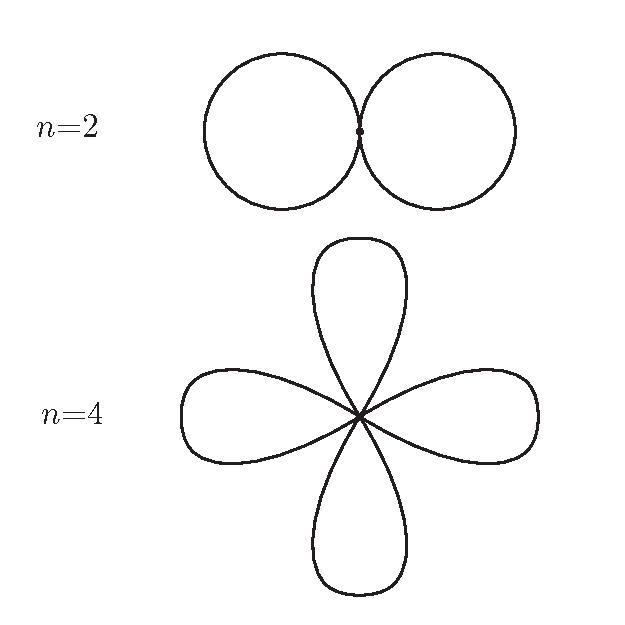
\includegraphics[trim=0cm 0cm 0cm 0cm,clip,scale=0.7]{images/bouquet.pdf}
\end{center}
\end{definition}
\begin{example}{pn}[Altri esempi di equivalenze omotopiche]~{}
	\begin{enumerate}
		\item $\R^2\setminus\left\{2\text{ punti}\right\}$ ha lo stesso tipo di omotopia di un \textit{bouquet di due circonferenze}: si può ottenere attraverso una composizione continua di retrazioni \textit{radiali} e \textit{lineari}\index{retrazione!lineare}.
		\begin{center}
						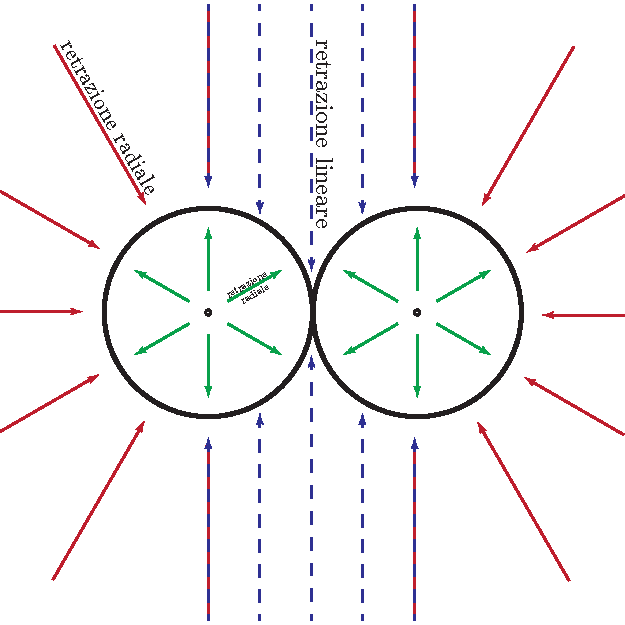
\includegraphics[trim=0cm 0cm 0cm 0cm,clip,scale=0.75]{images/bouquetconstruction.pdf}
		\end{center}	
		\item $\R^2\setminus\left\{n\text{ punti}\right\}$ ha lo stesso tipo di omotopia di un \textit{bouquet di} $n$ \textit{circonferenze}.
		\item $\R^3\setminus\left\{1\text{ retta}\right\}$ ha lo stesso tipo di omotopia di $\R^2\setminus\left\{1\ \text{punto}\right\}$ per retrazioni lineari, dunque ha la stessa omotopia di $S^1$ per i ragionamenti precedenti.
		\item Per $\R^3\setminus\left\{2\text{ rette}\right\}$ dobbiamo distinguere a seconda della relazione fra le due rette.
		\begin{itemize}
			\item Se le rette sono \textbf{disgiunte}, $X$ è sempre omeomorfo a
			\begin{equation*}
				\R^3\setminus\left\{\text{asse z}\right\}\setminus\left\{x=y=1\right\}\eqqcolon\widetilde{X},
			\end{equation*}
		cioè lo spazio $\R^3$ privato di due rette perpendicolari al piano $xy$ e distinte. Considerato ora $Y=\left\{\text{piano xy}\right\}\setminus\left\{\left(0,0\right),\ \left(1,1\right)\right\}$, questo risulta un retratto di deformazione di $\widetilde{X}$ con retrazione:
			\begin{equation*}
				\funct{}[r]{\widetilde{X}}{Y}[\left(x,\ y,\ z\right)][\left(x,\ y, 0\right)]
			\end{equation*}
		Infatti, la funzione è sempre ben definita, continua e, considerata la restrizione di $r$ ad $Y$, segue che banalmente che è l'identità di $Y$ in quanto tutti i punti di $Y$ hanno già la forma $\left(x,\ y, 0\right)$. Guardando invece $\widetilde{r}=i\circ r$ con $\funct{i}[i]{Y}{\widetilde{X}}$, un'omotopia con $Id_{\widetilde{X}}$ è
		\begin{equation*}
			\funct{}[F]{\widetilde{X}\times I}{\widetilde{X}}\ \colon F\left(\left(x,\ y,\ z\right),t\right)=\left(x,\ y,\ tz\right).
		\end{equation*}
		Infatti, $F$ è banalmente ben definita, continua e
		\begin{equation*}
			F\left(\mathbf{x},0\right)=\left(x,\ y,\ 0\right)=\widetilde{r}\left(\mathbf{x}\right)\qquad F\left(\mathbf{x},1\right)=\left(x,\ y,\ z\right)=Id_{\widetilde{X}}\left(\mathbf{x}\right).
		\end{equation*}
		Segue che $\widetilde{X}$, e dunque anche $X$ per omeomorfismo, ha la stessa omotopia di $\R^2\setminus\left\{2\text{ punti}\right\}$ e di un \textit{bouquet di due circonferenze}.
		\item Se le due rette sono \textbf{incidenti}, a meno di omeomorfismi si intersecano nell'origine. Consideriamo dunque $X=\R^3\setminus\left\{r_1\cup r_2\right\}$ e lo spazio $A=S^2\setminus\left\{P_1,\ P_2,\ Q_1,\ Q_2\right\}$. Se prendiamo la retrazione
		\begin{equation*}
			\funct{}[r]{X}{A}[\mathbf{x}][\frac{\mathbf{x}}{\norm{\mathbf{x}}}].
		\end{equation*}
		e l'omotopia
		\begin{equation*}
			\funct{}[\widetilde{r}\coloneqq i\circ r]{X}{X}[\mathbf{x}][\frac{\mathbf{x}}{\norm{\mathbf{x}}}]
		\end{equation*}
	si verifica in modo analogo a come visto nel caso della sfera e dello spazio privato dell'origine (esempio a pag. \pageref{retrattosfera}), trattando con una \textit{retrazione radiale} ben definita e la sua omotopia nota, che $A$ è retratto di deformazione di $X$. Segue allora che hanno lo stesso tipo di omotopia.
		\end{itemize}
	\end{enumerate}
\end{example}
